\chapter{Collision Handling with Penalty Methods}
\label{ch:DiscretePenaltyForces}
This chapter describes the collision handling with penalty methods.
We will first introduce the DPF and then extend the algorithm to a continuous formulation the CPF, taking the whole feature trajectory into account and thereby increasing stability and reducing jitter.
Afterwards, we present the penalty-based friction formulation.

Penalty methods handle constraints in a multi body system by applying forces opposed to the constraint violation to correct the velocity and position of the object. The strength of the force depends on the severeness of the constraint violation \cite{BENDER2007} and can be compared to a spring taking effect until the constraint is complied.

\section{Discrete Penalty Forces}
\label{sec:DiscretePF}
 The method of DPF defines a force field based on the penetration depth of two intersecting bodies. There are multiple definitions for penetration depth and the force field computation, we use the formulation presented by Tang et al. \cite{TANG2012}. For a point $\mathbf{x}$, belonging to object A and intersecting object B, the penetration depth $\delta(\mathbf{x})$ is defined as the distance to the closest point on the surface of B. Based on the penetration depth and the penalty coefficient $k$, the penalty energy is defined by
\begin{equation}
      E(\mathbf{x}) = \frac{1}{2}k \delta (\mathbf{x})^2 .
      \label{eq:penalty_energy}
\end{equation}
The formulation is similar to the energy $E_s(\mathbf x)$ of a spring system \cite{GROSS2011} %[p.224]
\begin{equation}
      E_{s}(\mathbf{x}) = \frac{1}{2} c ~||\mathbf{x-x_0}|| ^2,
\end{equation}
with the initial position $\mathbf x_0$ and the spring stiffness $c$.
The penalty coefficient $k$ corresponds to the spring stiffness $c$ and the penetration depth $\delta(\mathbf{x})$ corresponds to the spring expansion $||\mathbf{x-x_0}||$.
The penalty coefficient $k$ needs to be chosen in an empirical manner. According  its analogy to the spring stiffness, a similar behaviour can be observed. High penalty coefficients provide large contact forces and small intersections, however they also lead to unstable systems. On the other hand low penalty coefficients provide more stable systems with smaller forces but larger intersections. There is no exact rule how to choose the penalty coefficient, although we will show later (see section \ref{sec::stability}) that the relation $\Delta t \sim \sqrt{\frac{m}{k}}$ can be used as a rule of thumb.

According to the mechanical law of energy conservation \cite{WEBER2012} %[p.42]
 the  negative gradient of the penalty energy is the penalty force
\begin{equation}
      F(\mathbf{x}) = - \nabla  E(\mathbf{x})= - k \delta (\mathbf{x}) \nabla\delta (\mathbf{x}).
\end{equation}
With the definition of the penetration depth given above, the negative gradient of the penetration depth is equal to the unit surface normal $\mathbf{n}$ at the closest point on the surface of the penetrated object. The penalty force results in 
\begin{equation}
      F(\mathbf{x}) = k \delta (\mathbf{x}) \mathbf{n} 
            \label{eq:discrete_penalty_force}
\end{equation}
The impulse caused by DPF during a time step $\Delta t$ is the integral along time according to Newton's second law of motion
\begin{equation}
      I = \int_{t_i}^{t_i+\Delta t} F(\mathbf{x})dt=\Delta t F(\mathbf{x})=\Delta t k \delta (\mathbf{x}) \mathbf{n}. 
\end{equation}

The impulse can be applied to the vertices as described in section \ref{sec:InteractingRigDef}.

% !TeX spellcheck = en_GB
\section{Continuous Penalty Forces}
\label{sec:ContinuousPenaltyForces}
This section outlines the algorithm CPF presented by Tang et al. \cite{TANG2012}, which reduces instability and jitter in comparison to DPF and is the basis for this thesis. The general impulse formula for the vertex-face and edge-edge case will be derived and the exact formula for the case of linear interpolated trajectories will be presented.

\subsection{CCD and Penetration Depth}
\label{sec:CCDandPenetrationDepth}
To simplify the collision response with CPF, each simulation time step is normalized to the unit interval $[0, 1]$. The collisions are detected using a CCD algorithm, as described in section \ref{sec:CCD}, considering all possible pairwise features, VF and EE. Furthermore, the CCD provides the contact times for each feature pair and the collision points $\mathbf p(t)$ and $\mathbf q(t)$ at the first time-of-contact. The points $\mathbf p(t)$ and $\mathbf q(t)$ are traced along their trajectories until the collision is resolved.

In contrast to DPF, the penetration depth is defined by a formulation utilizing the information provided by CCD. A contact normal is defined for each contact pair. In the VF case, the time-dependent contact normal $\mathbf n(t)$ is the normal of the colliding triangle. In the EE case, the time-dependent contact normal $\mathbf n(t)$ is the cross product of the two edge vectors. The penetration depth is defined as the vector between the two contact points $\mathbf p(t)$ and $\mathbf q(t)$ projected onto the contact normal
\begin{equation}
       	\delta(t)  =\mathbf{n}(t) \cdot  (\mathbf p (t) - \mathbf q (t))
\end{equation}
A feature pair is considered colliding, from the first time of contact until the penetration depth is strictly positive. Within a normalized simulation time step the penetration time interval $[t^i_a , t^i_b] \in [0,1]$ is the interval in which the feature pair is colliding.
With linear trajectories, up to two penetration time intervals can occur within one time step, since the elementary collision test can return up to three real roots. For higher-degree trajectories even more time intervals can occur.

\subsection{Continuous Penalty Forces}
\label{sec:CPFGENERAL}
The CPF approach extends the idea of DPF and computes collision impulses by continuously accumulating penalty forces along the penetration depth over the whole time step. Thereby, not only the position at one moment but also the trajectory is included in the computation of the impulse.

The CPF $\mathbf F (t)$ is computed analogously to the DPF, but now with time-dependent definitions for the normal $\mathbf n (t)$, penetration depth $\mathbf{\delta}(t)$
\begin{equation}
    \mathbf  F(t) = k \delta (t) \mathbf{n} (t) = k\mathbf{n}(t) \cdot  (\mathbf p(t) - \mathbf q (t)) \mathbf{n} (t).
\end{equation}
The resulting impulse is computed with regard to the penetration intervals
\begin{equation}
\label{eq::CPF_impulse}
     \mathbf I = \int_{t_i}^{t_i+\Delta t} \mathbf F(t)dt= \sum\limits_{i=0}^{n}\int_{t_a^i}^{t_b^i}\mathbf F(t)dt=k \sum\limits_{i=0}^{n}\int_{t_a^i}^{t_b^i} \mathbf{n}(t) \cdot   (\mathbf p(t) - \mathbf q (t)) \mathbf{n} (t)dt.
\end{equation}
An illustration of the impulse computation is provided in figure \ref{fig:impulseComputationCPFDPF}. The linear trajectory can be approximated exactly by the CPF, see figure \ref{fig:impulseComputationCPFDPF} a) and c). Whereas, the DPF overestimate the penetration depth as long as the penetration depth is increasing, see figure \ref{fig:impulseComputationCPFDPF} b). The DPF underestimated the penetration depth as long as it is decreasing, see figure \ref{fig:impulseComputationCPFDPF} d).

\begin{figure}[h] 
  \centering
     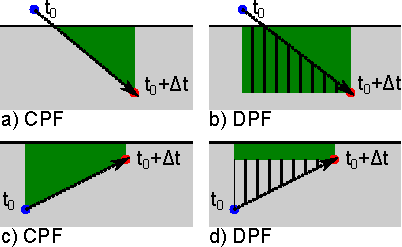
\includegraphics[width=0.7\textwidth]{pics/pdf/impulseComputationCPFDPF.pdf}
  \caption[2D Illustration of the resolution force computation for CPF and DPF in the VF case.]{2D Illustration of the resolution force computation for CPF and DPF in the VF case. The blue dot marks the position of the vertex of object A at the beginning of the time step and the red dot the predicted end position. The dotted arrow indicates the linearly approximated trajectory. The grey area is the inside of object B. The green area corresponds to the integral over the force and thereby the resolution impulse. The black striped areas indicate the estimation errors of the DPF forces. It is noticeable that the DPF overestimates the penetration depth as long as the penetration depth is increasing, see subfigure b), and underestimates the penetration depth as long as it is decreasing, see subfigure d).}
  \label{fig:impulseComputationCPFDPF}
\end{figure}

 
\subsection{Vertex-Face Contact Forces}
In the VF case, the contact point $\mathbf p(t)$ is the position of the colliding vertex V and  the contact point $\mathbf q(t)=\omega_a \mathbf a(t)+\omega_b \mathbf b(t)+\omega_c \mathbf c(t) $ is the representation of the collision point on the triangle T in barycentric coordinates with the vertex positions $\mathbf a$, $\mathbf b$ and $\mathbf c$ and their corresponding weights $\omega_a$, $\omega_b$ and $\omega_c$. The contact normal $\mathbf n_T(t) = (\mathbf b(t) - \mathbf a(t))\times(\mathbf c(t) - \mathbf a(t))$ is the normal of the triangle. With equation \ref{eq::CPF_impulse}, the impulse on the vertex p is
\begin{equation}
     \mathbf I_p =k \sum\limits_{i=0}^{n}\int_{t_a^i}^{t_b^i} \mathbf{n_T}(t) \cdot   (\mathbf p(t) - \omega_a \mathbf a(t)-\omega_b \mathbf b(t)-\omega_c \mathbf c(t)) \mathbf {n_T} (t)dt.
\end{equation}
The impulse on the triangle is distributed among the three vertices according to the barycentric weights

\begin{equation}
     \mathbf I_a =- \omega_a \mathbf I_p, 
     \mathbf I_b =- \omega_b \mathbf I_p,
     \mathbf I_c =- \omega_c \mathbf I_p.
\end{equation}
For linear interpolated motions, the velocity is constant and can be computed with the vertices' start and end position $\mathbf (\mathbf p_0,\mathbf p_1)$, $(\mathbf a_0,\mathbf a_1)$, $(\mathbf b_0,\mathbf b_1)$ and $(\mathbf c_0,\mathbf c_1)$ as $\mathbf v_p=\mathbf p_1-\mathbf p_0$ and similarly for $\mathbf v_a$, $\mathbf v_b$ and $\mathbf v_c$.
With the second order Bernstein polynomials
\begin{equation}
B^2_i(t)=\frac{2!}{i!(2-i)!}t^i(1-t)^{2-i}
\end{equation}
and the constant basis coefficients $\mathbf n_0=(\mathbf b_0- \mathbf a_0) \times (\mathbf c_0-\mathbf a_0)$, $\mathbf n_1= \frac{\mathbf n_0+ \mathbf n_2 - (\mathbf v_b-\mathbf v_a) \times (\mathbf v_c - \mathbf v_a)}{2}$ and $\mathbf n_2=(\mathbf b_1- \mathbf a_1) \times (\mathbf c_1-\mathbf a_1)$ and the normalization factor $L(t)$, the time varying contact normal is
\begin{equation}
	\mathbf{n_T}(t)=\frac{\mathbf{n_0}B^2_0(t)+\mathbf{n_1}B^2_1(t)+\mathbf{n_2}B^2_2(t)}{L(t)}.
\end{equation}
The normalization factor $L(t)$ is composed as
\begin{equation}
	L(t)=\sqrt{(L_0L_1...L_4)(B^4_0(t)B^4_1(t)...B^4_4(t))},
\end{equation}
with the factors $L_i$, which are given in the supplementary material of \cite{TANG2012}.


To compute the impulse exactly, it would be necessary to integrate the rational function $n_T$ which is rather complicated because of the denominator $L(t)$ \cite{TANG2012}.
Tang et al. suggest to approximate $L(t)$ by a constant $L_k$
\begin{equation}
	L(t)\approx L_k=\sqrt{\frac{L_0+L_1+L_2+L_3+L_4}{5}}.
\end{equation}
With this approximation the normal is a quadratic term and the computation of the integral is simplified, resulting in speed-ups up to an order of magnitude without noticeable differences in the simulation results \cite{TANG2012}.

\subsection{Edge-Edge Contact Forces}
In the EE case, the contact points $\mathbf p(t)=\omega_a \mathbf a(t)+\omega_b \mathbf b(t)$ and $\mathbf q(t)=\omega_c \mathbf c(t)+\omega_d \mathbf d(t) $ are the barycentric representation of the collision points on the edges $E_1$ and $E_2$ with the vertex positions $\mathbf a(t)$, $\mathbf b(t)$, $\mathbf c(t)$ and $\mathbf d(t)$ and their corresponding weights $\omega_a$, $\omega_b$, $\omega_c$ and $\omega_d$.
The contact normal $\mathbf{ n_E}(t) = (\mathbf b(t) - \mathbf a(t))\times(\mathbf d(t) - \mathbf c(t))$ is the cross product of the two edge vectors.  With equation \ref{eq::CPF_impulse} the impulse on the edge $E_1$ is
\begin{equation}
     \mathbf I_E =k \sum\limits_{i=0}^{n}\int_{t_a^i}^{t_b^i} \mathbf{n_E}(t) \cdot   (\omega_a \mathbf a(t)+\omega_b \mathbf b(t)-\omega_c \mathbf c(t)-\omega_d \mathbf d(t)) \mathbf {n_E} (t)dt.
\end{equation}
The impulse is distributed among the four vertices according to the barycentric weights
\begin{equation}
     \mathbf I_a = \omega_a \mathbf I_E, 
     \mathbf I_b = \omega_b \mathbf I_E,
     \mathbf I_c =- \omega_c \mathbf I_E,
     \mathbf I_d =- \omega_d \mathbf I_E.
\end{equation}
Similar to the VF case, for linear interpolated motion the velocity is constant and the velocity can be computed from the vertices' start and end positions  $(\mathbf a_0,\mathbf a_1)$, $(\mathbf b_0,\mathbf b_1)$, $(\mathbf c_0,\mathbf c_1)$  and $(\mathbf d_0,\mathbf d_1)$ as $\mathbf v_a=\mathbf a_1-\mathbf a_0$ and analogously for $\mathbf v_b$, $\mathbf v_c$ and $\mathbf v_d$. With the second order Bernstein polynomials 
\begin{equation}
B^2_i(t)=\frac{2!}{i!(2-i)!}t^i(1-t)^{2-i}
\end{equation}
and the constant basis coefficients $\mathbf n'_0=(\mathbf b_0- \mathbf a_0) \times (\mathbf d_0-\mathbf c_0)$, $\mathbf n'_1= \frac{\mathbf n'_0+ \mathbf n'_2 - (\mathbf v_b-\mathbf v_a) \times (\mathbf v_d - \mathbf v_c)}{2}$ and $\mathbf n'_2=(\mathbf b_1- \mathbf a_1) \times (\mathbf d_1-\mathbf c_1)$ and the normalization factor $L(t)$, the time varying contact normal can be expressed as

\begin{equation}
	\mathbf{n_T}(t)=\frac{\mathbf n'_0 B^2_0(t)+\mathbf n'_1 B^2_1(t)+\mathbf n'_2 B^2_2(t)}{L(t)}
\end{equation}
The normalization factor $L(t)$ can be computed as in the VF case.


We now give an example how to apply CPF for collisions for a static ground plane.
Ground collisions are a common scenario in many environments and due to the static plane the formula can be simplified.

 For collisions with the ground plane in an environment with gravity in the negative y-direction, the contact normal $\mathbf{n_P}=(0,1,0)$ is constant. With the position of the colliding vertex $\mathbf p(t)$ the impulse is

\begin{equation}
     \mathbf I_p =k \sum\limits_{i=0}^{n}\int_{t_a^i}^{t_b^i} \mathbf{n_P} \cdot   \mathbf p(t) \mathbf {n_P}dt=k \sum\limits_{i=0}^{n}\int_{t_a^i}^{t_b^i} (0,p_y(t),0)  dt,
\end{equation}
with $p_y(t)$ the $\mathbf p(t)$ component in $y$-direction.

Again we assume linear interpolated motion for the particle $\mathbf p(t)= \mathbf{p_0}+t \mathbf{v_p}$. Solving the integral gives a quadratic expression for the vertex impulse
\begin{equation}
 \mathbf I_p=(0,(t_a-t_b) kp_y(t_0)-\frac{t_b^2-t_a^2}{2} kv_y,0).
\end{equation}
No outer sum is required, since maximum one penetration interval can occur.
%Since we only detect and handle vertex-ground collisions, it is necessary to compensate the potential edge-ground forces by the vertex-ground for to reach a consistent contact handling in the scene. Otherwise the body-body collisions are stiffer than the body-ground collisions. The ratio of vertices to edges, was for multiple tested meshes $1:2.98 \pm 0.03$, see appendix \ref{TODO}, giving us a compensation factor of $1+2.98\approx4$. For ground collisions we compute the impulse with a modified stiffness coefficient $k^*=4k$ resulting in an new impulse
%\begin{equation}
%     \mathbf I_p^* =k^* \sum\limits_{i=0}^{n}\int_{t_a^i}^{t_b^i} (0,p_y(t),0)\cdot dt
%\end{equation}

\section{Friction}
\label{ch:Friction}
We model friction with a penalty-based model by Yamane and Nakamura\cite{YAMANE2006}, providing a straightforward integration in the penalty based collision resolution, only small computational overhead and an unified handling for rigid and deformable bodies. The penalty-based formulation differs between dynamic and static friction, similar to  Coulomb's friction law. 
Coulomb's friction law \cite{YAMANE2006} defines the friction force $\mathbf f_f$ as
\begin{equation}
\mathbf f_f=
\begin{cases}
\mathbf f_s & \text{ if } |v_{slip}|=0 \text{ and } |\mathbf f_{s}|\le\mu_S |\mathbf f_n| \\
\mu_D \mathbf f_n & \text{ else }
\end{cases}
\end{equation}
with the static and dynamic friction coefficients $\mu_s$ and $\mu_d$ and the normal force $\mathbf f_n$.
For the model by Yamane and Nakamura, we first compute the static friction force $\mathbf f_s$ as
\begin{equation}
\mathbf f_s= (k_{FP}(\mathbf p_{ref} - \mathbf p)-k_{FD}\mathbf v_{slip} )
\end{equation}
with the penalty coefficients $k_{FP}$ and $k_{FD}$, the current position $\mathbf p$ and the reference position $\mathbf p_{ref}$, where $\mathbf p$ is to be fixed. $\mathbf p_{ref}$ is initialized when the features come into contact with the contact point and is updated to the current position $\mathbf p$ each time dynamic friction is applied. Similar to Coulombs law, we apply static friction, if $|\mathbf f_s|\le\mu_s|\mathbf f_n|$. Otherwise we apply dynamic friction as
\begin{equation}
\mathbf f_d=-\mu_d |\mathbf f_n| \frac{\omega (|\mathbf{v}_{slip}|)}{|\mathbf{v}_{slip}|}\mathbf{v}_{slip},
\end{equation}\\
with the continuous weighting function $\omega(x)$.  $\omega(x)$ is defined by
\begin{equation}
\omega(x)=1-e^{-k_\omega x}
\end{equation}
with the positive constant $k_\omega$. $\omega (x)$ satisfies $\omega(0)=0$ and $\lim_{x \rightarrow + \infty}\omega(x)=1$. Furthermore, $\omega(x)$ solves the potential singularity arising from the division by $|\mathbf v_{slip}|$ for small $|\mathbf{v}_{slip}|$, since 
\begin{equation}
\lim\limits_{x\rightarrow 0}\frac{\omega (x)}{x}=k_{\omega}.
\end{equation}
Therby, for $|v_{slip}| \ll 1$ the dynamic friction can be approximated as
\begin{equation}
\mathbf f_d=-\mu_d |\mathbf f_n| k_{\omega}\mathbf{v}_{slip}.
\end{equation}


The static friction model is similar to applying a damped spring at the contact point. If the spring force is too large, dynamic friction is applied.